\documentclass[11pt]{beamer}
\usetheme{CambridgeUS}
\usepackage[utf8]{inputenc}
\usepackage{amsmath}
\usepackage{amsfonts}
\usepackage{amssymb}
\usepackage[
backend=biber,
style=alphabetic,
citestyle=authoryear
]{biblatex}
\usepackage{array}
\usepackage{xcolor}

% Footnote without number
\newcommand\blfootnote[1]{%
  \begingroup
  \renewcommand\thefootnote{}\footnote{#1}%
  \addtocounter{footnote}{-1}%
  \endgroup
}
\def\boxit#1{%
  \smash{\color{red}\fboxrule=1pt\relax\fboxsep=2pt\relax%
  \llap{\rlap{\fbox{\vphantom{0}\makebox[#1]{}}}~}}\ignorespaces
}
\addbibresource{stats.bib}
\title[Bioestatística II] %optional
{Estimativa com Intervalos de confiança}

\subtitle{CGF2046 - Bioestatística II}

\author[da Silva, Ricardo] % (optional, for multiple authors)
{R. ~R. ~da Silva\inst{1}}

\institute[FCFRP] % (optional)
{
  \inst{1}%
  Departamento de Ciências BioMoleculares\\
  Faculdade de Ciências Farmacêuticas

}

\date{\today} % (optional)

\titlegraphic{
\includegraphics[width=5.8cm]{figs/logo_final}} 

\begin{document}

%\begin{frame}
%\titlepage
%\end{frame}

%\begin{frame}
%\tableofcontents
%\end{frame}

\begin{frame}
\titlepage
\end{frame}

\begin{frame}
\label{contents}
\frametitle{Sumário}
\tableofcontents
\end{frame}

\setbeamercovered{transparent}
\begin{frame}
\frametitle{Objetivos de Aprendizado\footcite{carlson2017introduction}}
  Depois de assitir essa aula e fazer as atividades complementares, você será capaz de:
  \\~\\
  \begin{itemize}
  \uncover<1->{\item
    Descrever os objetivos distintos dos testes de significância, tamanhos de efeito e intervalos de confiança;}
  \uncover<2->{\item
    Explique a lógica dos intervalos de confiança;}
   \uncover<3->{\item
    Calcular um intervalo de confiança para uma média populacional;}
   \uncover<4->{\item
    Calcular um intervalo de confiança para uma diferença média entre uma média amostral e uma média populacional;}
   \uncover<5->{\item
    Relatar intervalos de confiança;}
   \uncover<6->{\item
    Identificar interpretações corretas e incorretas de intervalos de confiança.}     
  \end{itemize}
\end{frame}

\section{Introdução ao teste t}
\setbeamercovered{transparent}
\begin{frame}
\frametitle{Contexto}
No Capítulo 7, você aprendeu como usar o teste t de amostra única para determinar 
\begin{itemize}
\item se uma diferença observada entre uma média amostral e uma média populacional tem probabilidade de ser criada por erro amostral ou por uma variável independente (VI; ou seja, o variável de agrupamento); 
\item e o tamanho do efeito (d) para descrever a magnitude do impacto do VI na variável dependente (VD).
\end{itemize}

\end{frame}


\setbeamercovered{transparent}
\begin{frame}
\frametitle{Três procedimentos estatísticos com três finalidades distintas}

\textbf{Exemplo:} O reitor de uma faculdade está considerando adicionar uma aula de "vida saudável" aos requisitos de educação geral para os alunos, mas primeiro pretende determinar se frequentar tal aula aumenta os comportamentos saudáveis,

\begin{itemize}
\item A reitoria entrevistou toda a população de estudantes e constatou que eles relataram praticar exercícios em média 150 minutos por semana;
\item Foram recrutados 60 estudantes universitários que frequentaram o novo curso. Depois de concluírem a aula, os participantes usaram um monitor de frequência cardíaca durante 1 mês;
\item O resultado do teste t para amostra única: \(t_{(59)} = 2.11\), p = 0.04 (o valor p bicaudal tem que ser multiplicado por dois quando calculado), d = 0.27.
\end{itemize}

\end{frame}

\setbeamercovered{transparent}
\begin{frame}
\frametitle{Três procedimentos estatísticos com três finalidades distintas}

A melhor estimativa deste parâmetro é a média da amostra que realizou a aula - ou seja, 155.67 minutos. No entanto, devido ao erro amostral, esta média amostral provavelmente não é perfeitamente precisa.\\~\\

Um intervalo de confiança é um procedimento estatístico que utiliza a mesma fórmula de erro amostral esperado (isto é, \(SEM_a\)) que os testes de hipóteses, mas de uma maneira diferente, para criar um intervalo de valores plausíveis para o parâmetro populacional.

\end{frame}

\setbeamercovered{transparent}
\begin{frame}
\frametitle{Estimação}

Por serem \textbf{variáveis aleatórias}, os estimadores pontuais possuem
uma distribuição de probabilidade (distribuições amostrais).

Com isso, podemos apresentar uma estimativa mais informativa para o
parâmetro de interesse, que inclua uma medida de \textbf{precisão} do
valor obtido \(\rightarrow\) \textbf{estimativa intervalar} ou
\textbf{intervalo de confiança}.

Os \textbf{intervalos de confiança} são obtidos a partir da
\textbf{distribuição amostral} de seus estimadores.
\end{frame}

\section{Intervalos de confiança: \(\sigma\) conhecido}
\setbeamercovered{transparent}
\begin{frame}
\frametitle{Suposições necessárias}

\begin{itemize}
\item
  A amostra é uma \textbf{amostra aleatória simples}. (Todas as amostras
  de mesmo tamanho tem a mesma probabilidade de serem selecionadas)
\item
  O valor do desvio padrão populacional \(\sigma\), é conhecido
\item
  Uma ou ambas das seguintes condições são satisfeitas:

  \begin{itemize}
  \item
    A população é normalmente distribuída
  \item
    A amostra possui \(n > 30\)
  \end{itemize}
\end{itemize}
\end{frame}

\setbeamercovered{transparent}
\begin{frame}
\frametitle{Erro amostral}

Quando coletamos uma \textbf{amostra aleatória} e calculamos uma média,
sabemos que o valor da média possui um desvio natural, em relação ao
verdadeiro valor da média populacional (\textbf{erro amostral}), ou seja
\[
e = \bar{X} - \mu \quad \Rightarrow \quad \bar{X} = \mu + e
\]

Sabemos que a \textbf{distribuição amostral da média} é uma distribuição
normal, com média \(\mu\) e variância \(\sigma^2/n\), \[
\bar{X} \sim \text{N}\left(\mu, \frac{\sigma^2}{n}\right)
\]
\end{frame}

\setbeamercovered{transparent}
\begin{frame}
\frametitle{Margem de erro}

Usando a transformação \[
Z = \frac{\bar{X} - \mu}{\sigma/\sqrt{n}} =
\frac{e}{\sigma/\sqrt{n}} \, \sim \, \text{N}(0,1)
\] podemos determinar o \textbf{erro máximo provável} que assumimos para
a média amostral que estamos calculando.

O \textbf{erro máximo provável} ou \textbf{margem de erro} da média é
definido por \[
e = z_{\gamma/2} \cdot \frac{\sigma}{\sqrt{n}}
\] onde \(z_{\gamma/2}\) é chamado de \textbf{valor crítico}.
\end{frame}


\setbeamercovered{transparent}
\begin{frame}
\frametitle{Intervalo de confiança}

Fixando um valor \(\gamma\) tal que \(0 < \gamma < 1\), podemos
encontrar um valor \(z_{\gamma/2}\) tal que:

\begin{align*}
&P[|Z| < z_{\gamma/2}] &= \gamma \\
&P[-z_{\gamma/2} < Z < z_{\gamma/2}] &= \gamma \\
&P[-z_{\gamma/2} < \frac{\bar{x} - \mu}{\sigma/\sqrt{n}} <
z_{\gamma/2}] &= \gamma \\
&P[\bar{x} - z_{\gamma/2} \cdot
\left(\frac{\sigma}{\sqrt{n}} \right) < \mu < \bar{x} + z_{\gamma/2}
\cdot \left(\frac{\sigma}{\sqrt{n}} \right)] &= \gamma \\
&P[\bar{x} - e < \mu < \bar{x} + e] &= \gamma \\
\end{align*}
\end{frame}

\setbeamercovered{transparent}
\begin{frame}
\frametitle{Intervalo de confiança}

O valor crítico \(z_{\gamma/2}\) é o valor de \(\gamma\) dividido por 2,
uma vez que a ``massa'' \(\gamma\) deve ser distribuída igualmente em
torno de 0.

\begin{center}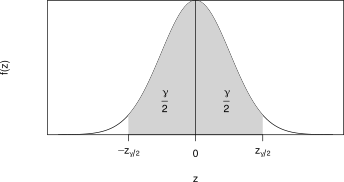
\includegraphics[width=0.8\linewidth]{figs/unnamed_chunk_1_1} \end{center}
\end{frame}

\setbeamercovered{transparent}
\begin{frame}
\frametitle{Coeficiente de confiança \(\gamma\)}

A área \(\gamma\) determina o \textbf{coeficiente de confiança}
associado ao intervalo de confiança que estamos construindo.

O valor \(z_{\gamma/2}\) pode ser obtido da tabela da Normal padrão,
localizando o valor de \(\gamma/2\) no corpo da tabela e obtendo o valor
\(z_{\gamma/2}\) nas margens correspondentes.

Exemplo: \(\gamma = 0,95\):

\begin{itemize}
\item
  Temos que \(\gamma/2 = 0,475\) é a área que devemos procurar no corpo
  da tabela
\item
  O valor de \(z_{\gamma/2}\) será determinado pelos valores
  correspondentes nas margens da tabela. Nesse caso,
  \(z_{\gamma/2} = 1,96\) é o valor crítico procurado.
\end{itemize}
\end{frame}

\setbeamercovered{transparent}
\begin{frame}
\frametitle{Intervalo de confiança}

Com estas definições, podemos construir um \textbf{intervalo de
confiança} para \(\mu\), com \textbf{coeficiente de confiança}
\(\gamma\): \[
\text{IC}(\mu, \gamma) = \left[ \bar{X} - z_{\gamma/2} \cdot
  \left(\frac{\sigma}{\sqrt{n}}\right) ; \bar{X} + z_{\gamma/2} \cdot
  \left(\frac{\sigma}{\sqrt{n}}\right)  \right]
\]

Outras notações: \[\bar{x} - e < \mu < \bar{x} + e\] \[\bar{x} \pm e\]
\[[\bar{x} - e; \bar{x} + e]\]
\end{frame}

\setbeamercovered{transparent}
\begin{frame}
\frametitle{Procedimentos gerais para a construção de intervalos de confiança}

\begin{enumerate}
\def\labelenumi{\arabic{enumi}.}
\item
  Verifique se as suposições necessárias estão satisfeitas

  \begin{itemize}
  \item
    Temos uma AAS
  \item
    \(\sigma\) é conhecido
  \item
    A população tem distribuição normal ou \(n>30\)
  \end{itemize}
\item
  Determine o nível de confiança \(\gamma\), e encontre o valor crítico
  \(z_{\gamma/2}\)
\item
  Calcule a margem de erro \(e = z_{\gamma/2} \cdot (\sigma/\sqrt{n})\)
\item
  Calcule \(\text{IC}(\mu, \gamma)\)
\end{enumerate}
\end{frame}

\setbeamercovered{transparent}
\begin{frame}
\frametitle{Interpretação de um intervalo de confiança}

Suponha que obtivemos um intervalo de 95\% de confiança:
\(\text{IC}(\mu,95\%) = [52; 58]\)

\begin{block}{Interpretação 1}
Temos 95\% de confiança de que a verdadeira média populacional $\mu$
se encontra entre 52 e 58
\end{block}
\begin{block}{Interpretação 2}
Temos 95\% de confiança de que o intervalo entre 52 e 58 realmente
contém a verdadeira média populacional $\mu$
\end{block}
\end{frame}

\setbeamercovered{transparent}
\begin{frame}
\frametitle{Interpretação de um intervalo de confiança}

Suponha que obtivemos um intervalo de 95\% de confiança:
\(\text{IC}(\mu,95\%) = [52; 58]\)

\begin{alertblock}{Interpretação 1 --- ERRADA}
Temos 95\% de confiança de que a verdadeira média populacional $\mu$
se encontra entre 52 e 58
\end{alertblock}
\begin{block}{Interpretação 2 --- CERTA}
Temos 95\% de confiança de que o intervalo entre 52 e 58 realmente
contém a verdadeira média populacional $\mu$
\end{block}
\end{frame}

\setbeamercovered{transparent}
\begin{frame}
\frametitle{Interpretação de um intervalo de confiança}

Como o intervalo de confiança é calculado a partir de uma
\textbf{amostra aleatória}, este intervalo \textbf{também é aleatório}!

Isso significa que para cada amostra aleatória que tivermos, um
intervalo \textbf{diferente} será calculado.

Como o valor de \(\mu\) é fixo, é o intervalo que deve conter o valor de
\(\mu\), e não o contrário.

Isso significa que se pudessemos obter 100 amostras diferentes, e
calcularmos um intervalo de confiança de 95\% para cada uma das 100
amostras, esperariamos que 5 destes intervalos \textbf{não} contenham o
verdadeiro valor da média populacional \(\mu\).
\end{frame}

\setbeamercovered{transparent}
\begin{frame}
\frametitle{Interpretação de um intervalo de confiança}

\begin{center}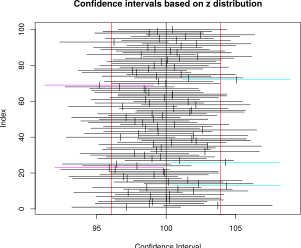
\includegraphics[width=0.7\linewidth]{figs/unnamed_chunk_2_1} \end{center}
\end{frame}


\setbeamercovered{transparent}
\begin{frame}
\frametitle{Amplitude de um intervalo}

A \textbf{amplitude} de um intervalo de confiança é dada pela diferença
entre o limite superior e inferior, ou seja, \begin{align*}
\text{AMP}_{IC} &=
  \left[ \bar{x} + z_{\gamma/2} \cdot
  \left( \frac{\sigma}{\sqrt{n}} \right) \right] -
  \left[ \bar{x} - z_{\gamma/2} \cdot
  \left( \frac{\sigma}{\sqrt{n}} \right) \right] \\
 &= 2 \times z_{\gamma/2} \cdot (\sigma/\sqrt{n})
\end{align*}

\begin{itemize}
\item
  Note que, claramente, um intervalo de confiança depende conjuntamente
  de três componentes:

  \begin{itemize}
  \item
    Coeficiente de confiança \(\gamma\), expresso pelo valor crítico
    \(z_{\gamma/2}\)
  \item
    Desvio-padrão populacional \(\sigma\)
  \item
    Tamanho da amostra \(n\)
  \end{itemize}
\end{itemize}
\end{frame}

\setbeamercovered{transparent}
\begin{frame}
\frametitle{Amplitude de um intervalo}

\(z_{\gamma/2} \rightarrow\) Cada vez que aumentamos a confiança
\(\gamma\), o valor de \(z_{\gamma/2}\) fica maior, e consequentemente a
amplitude do intervalo aumenta.

\(\sigma \rightarrow\) Um grande desvio padrão indica a possibilidade de
um considerável distanciamento dos valores amostrais em relação à média
populacional

\(n \rightarrow\) Quanto maior for o tamanho da amostra, maior será a
quantidade de informação disponível. Com isso, valores maiores de \(n\)
produzem intervalos mais informativos
\end{frame}


\section{Intervalos de confiança: \(\sigma\) desconhecido}
\setbeamercovered{transparent}
\begin{frame}
\frametitle{Determinação do tamanho amostral}

Nosso objetivo é coletar dados para estimar a \textbf{média
populacional} \(\mu\).

A questão é:

\begin{quote}
\textbf{Quantos elementos (itens, objetos, pessoas, \ldots{}) devemos
amostrar?}
\end{quote}

Já vimos que, de maneira (bem) geral, \(n>30\) é um tamanho de amostra
mínimo para a maioria dos casos.

Será que podemos ter uma estimativa melhor de quantos elementos devem
ser amostrados para estimarmos a média populacional com uma precisão
conhecida?
\end{frame}

\setbeamercovered{transparent}
\begin{frame}
\frametitle{Determinação do tamanho amostral}

A partir da equação do \textbf{erro máximo provável} \[
e = 2 z_{\gamma/2} \cdot \frac{\sigma}{\sqrt{n}}
\] podemos isolar \(n\) e chegar na seguinte equação para a determinação
do tamanho amostral \[
n = \left[ \frac{2 z_{\gamma/2} \cdot \sigma}{e} \right]^2
\]
\end{frame}

\setbeamercovered{transparent}
\begin{frame}
\frametitle{Determinação do tamanho amostral}

Note que, em \[
n = \left[ \frac{2 z_{\gamma/2} \cdot \sigma}{e} \right]^2
\]

\begin{itemize}
\item
  O tamanho amostral \(n\) \textbf{não} depende do tamanho populacional
  \(N\)
\item
  O tamanho amostral depende:

  \begin{itemize}
  \item
    do nível de confiança desejado (expresso pelo valor crítico
    \(z_{\gamma/2}\))
  \item
    do erro máximo \textsl{desejado}
  \item
    do desvio-padrão \(\sigma\) (embora veremos que não é estritamente
    necessário)
  \end{itemize}
\item
  Como o tamanho amostral precisa ser um número inteiro, arredondamos
  sempre o valor para o \textbf{maior} número inteiro mais próximo
\end{itemize}
\end{frame}

\setbeamercovered{transparent}
\begin{frame}
\frametitle{Cálculo do intervalo de confiança}

Com estas definições, podemos construir um \textbf{intervalo de
confiança} para \(\mu\), com \textbf{coeficiente de confiança}
\(\gamma\), com variância desconhecida, é dado por: \[
\text{IC}(\mu, \gamma) = \left[ \bar{X} - t_{\gamma/2} \cdot
  \left(\frac{S}{\sqrt{n}}\right) ; \bar{X} + t_{\gamma/2} \cdot
  \left(\frac{S}{\sqrt{n}}\right)  \right]
\]
Outras notações:
\[\text{IC}(\mu, \gamma) = \left[ \bar{X} - t_{IC} \cdot
  \left(SEM_a\right) ; \bar{X} + t_{IC} \cdot
  \left(SEM_a\right)  \right]
\]
\end{frame}

\setbeamercovered{transparent}
\begin{frame}
\frametitle{Cálculo do intervalo de confiança}

Agora, o reitor quer aplicar esses resultados da pesquisa à população de seu interesse, calculando um IC de 95\% para estimar esse parâmetro populacional. Comece escrevendo as seguintes fórmulas para os limites superior e inferior do IC.\\~\\

Para o cálculo você precisa dos mesmos três valores: 
\begin{itemize}
\item a estimativa pontual ou $\bar{x}$;
\item o valor t crítico correto para o IC ou $t_{IC}$;
\item o erro de amostragem esperado ou $SEM_a$.
\end{itemize}

O valor t crítico vem da tabela t crítica bicaudal 0.05 porque estamos computando um IC de 95\% de confiança. O \textit{gl} é 59 (gl = n - 1 = 60 - 1 = 59), então o \(t_{IC}\) é 2.001. E os \(SEM_a\) é \(DP/\sqrt{N}\) ou 20.85/60 = 2.69.

\end{frame}

\setbeamercovered{transparent}
\begin{frame}
\frametitle{Cálculo do intervalo de confiança}

Portanto, o limite superior do IC de 95\% é

\[Limite\quad superior = 155.67 + (2.001)(2.69) = 161.05\]

O limite inferior é

\[Limite\quad inferior = 155.67 - (2.001)(2.69) = 150.29\]

Levando ao intervalo

\[\text{IC}(\mu, 95\%) = [150.29, 161.05]\]

Com base nestes cálculos, deveríamos ter 95\% de confiança de que o intervalo 150.29 e 161.05 minutos por semana, contém o tempo médio real de exercício da população de estudantes universitários, se participassem nas aulas de vida saudável.
\end{frame}

\setbeamercovered{transparent}
\begin{frame}
\frametitle{Computação de intervalos de confiança para uma diferença média}

A única diferença entre este IC e o calculado acima é que estamos usando uma diferença entre uma média amostral e uma média populacional como estimativa pontual, em vez da média amostral em si. Os limites superior e inferior são calculados da seguinte forma:

Limite = Estimativa pontual +/- Margem de erro.

\begin{align*}
Limite\quad superior = (\bar{x}-\mu) + t_{IC}SEM_a\\ 
Limite\quad superior = (155.67 - 150) + (2.001)(2.69).\\
Limite\quad superior = 5.67+5.383 = 11.05.\\
Limite\quad superior = (\bar{x}-\mu) - t_{IC}SEM_a\\
Limite\quad inferior = (155.67 - 150) - (2.001)(2.69).\\
Limite\quad inferior = 5.67-5.383 = 0.29.\\
\end{align*}

\end{frame}

\setbeamercovered{transparent}
\begin{frame}
\frametitle{Computação de intervalos de confiança para uma diferença média}

Com base nestes cálculos, deveríamos ter 95\% de confiança de que o tempo de exercício por semana aumentaria entre 0.29 e 11.05 minutos se a população de estudantes universitários frequentasse as aulas de vida saudável. \\~\\

A regra geral é que os valores de IC tornam-se menos plausíveis com o aumento da distância da estimativa pontual.\\~\\

Se uma diferença média de zero não estiver entre os limites superior e inferior do IC de 95\% para a diferença média, a média amostral de 155.67 e a média populacional de 150 são significativamente diferentes uma da outra, se você realizar um teste de significância bicaudal com um valor alfa de 0.05.

\end{frame}

\setbeamercovered{transparent}
\begin{frame}
\frametitle{Relatório de intervalos de confiança}

Recomenda se que os pesquisadores calculem e interpretem os ICs em conjunto com testes de significância e tamanhos de efeito ao relatar resultados. 

Um teste t de amostra única revelou que os alunos que frequentaram o curso de vida saudável se exercitavam mais semanalmente (\(\bar{x} = 155.67\), DP = 2.69), \(IC(\mu, 95\%)= [150,29, 161,05]\), do que os alunos da população ($\mu = 150$), $t_{(59)} = 2.11$, p = 0.04, d = 0.27.

\end{frame}

\begin{frame}
\frametitle{Distribuição Normal}

\begin{center}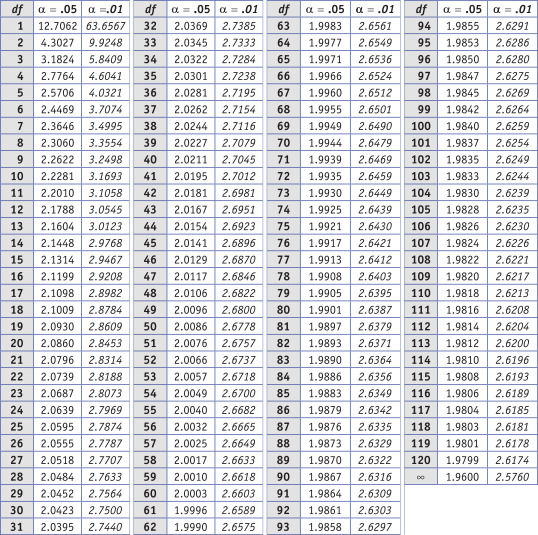
\includegraphics[width=0.7\linewidth]{figs/tabela_t} \end{center}
\end{frame}


\setbeamercovered{transparent}
\begin{frame}
\frametitle{Exemplo 8.6}
Deseja-se investigar se uma certa moléstia que ataca o rim altera o consumo de oxigênio desse orgão. Foram obtidos \(\bar{x}=13.9\) e \(Var(X)=0.67\). Determine o intervalo de confiança para \(\mu\) com \(\gamma=0.95\).
\vspace{1in}
\vspace{1in}

\end{frame}

\setbeamercovered{transparent}
\begin{frame}
\frametitle{Exemplo 10.5\footcite{martinez2015bioestatistica}}
Em um estudo sobre a deficiência de zinco em crianças, foi utilizada uma amostra de \(n=35\) crianças. Em amostras de sangue dessas crianças, obtidas por punção venosa, foi encontrada uma média de \(\bar{x}=118.7\ \mu g/dl\) para os níveis séricos de zinco, com desvio padrão amostral de \(DP=23.1 \mu g/dl\). Determine o intervalo de confiança para \(\mu\) com \(\gamma=0.99\).
\vspace{1in}
\vspace{1in}

\end{frame}


\setbeamercovered{transparent}
\begin{frame}
\frametitle{Referências bibliográficas}
\printbibliography
\end{frame}

\end{document}